%%%%%%%%%%%%%%%%%%%%%%%%%%%%%%%%%%%%%
%                                   %
% Compile with XeLaTeX and biber    %
%                                   %
% Questions or comments:            %
%                                   %
% joshua dot mcneill at uga dot edu %
%                                   %
%%%%%%%%%%%%%%%%%%%%%%%%%%%%%%%%%%%%%

\documentclass{beamer}
  % Read in standard preamble (cosmetic stuff)
  %%%%%%%%%%%%%%%%%%%%%%%%%%%%%%%%%%%%%%%%%%%%%%%%%%%%%%%%%%%%%%%%
% This is a standard preamble used in for all slide documents. %
% It basically contains cosmetic settings.                     %
%                                                              %
% Joshua McNeill                                               %
% joshua dot mcneill at uga dot edu                            %
%%%%%%%%%%%%%%%%%%%%%%%%%%%%%%%%%%%%%%%%%%%%%%%%%%%%%%%%%%%%%%%%

% Beamer settings
% \usetheme{Berkeley}
\usetheme{CambridgeUS}
% \usecolortheme{dove}
% \usecolortheme{rose}
\usecolortheme{seagull}
\usefonttheme{professionalfonts}
\usefonttheme{serif}
\setbeamertemplate{bibliography item}{}

% Packages and settings
\usepackage{fontspec}
  \setmainfont{Charis SIL}
\usepackage{hyperref}
  \hypersetup{colorlinks=true,
              allcolors=blue}
\usepackage{graphicx}
  \graphicspath{{../../figures/}}
\usepackage[normalem]{ulem}
\usepackage{enumerate}

% Document information
\author{M. McNeill}
\title[FREN2001]{Français 2001}
\institute{\url{joshua.mcneill@uga.edu}}
\date{}

%% Custom commands
% Lexical items
\newcommand{\lexi}[1]{\textit{#1}}
% Gloss
\newcommand{\gloss}[1]{`#1'}
\newcommand{\tinygloss}[1]{{\tiny`#1'}}
% Orthographic representations
\newcommand{\orth}[1]{$\langle$#1$\rangle$}
% Utterances (pragmatics)
\newcommand{\uttr}[1]{`#1'}
% Sentences (pragmatics)
\newcommand{\sent}[1]{\textit{#1}}
% Base dir for definitions
\newcommand{\defs}{../definitions}


  % Packages and settings

  % Document information
  \subtitle[Passé composé (\lexi{être})]{Le passé composé avec \lexi{être} et plus d'aliments}

\begin{document}
  % Read in the standard intro slides (title page and table of contents)
  \begin{frame}
    \titlepage
    \tiny{Office: % Basically a variable for office hours location
Gilbert 121\\
          Office hours: % Basically a variable for office hours
 lundi, mercredi, vendredi 10:10--11:10
}
  \end{frame}

  \begin{frame}{Annonces}
    \begin{itemize}
      \item Pas d'heures de permanence jeudi. Mardi, les heures prolongée de 1h30 à 4h30
      \item[] \tinygloss{No office hours Thursday. Tuesday, office hours extended from 1:30 to 4:30}
      \item L'atelier d'écriture vendredi
      \item[] \tinygloss{Writing workshop Friday}
    \end{itemize}
  \end{frame}

  \begin{frame}{}
    \begin{center}
      \Large Quiz
    \end{center}
  \end{frame}

  \begin{frame}{La structure et les verbes}
    \begin{center}
      sujet $+$ \lexi{être} (conjugated) $+$ participle (with agreement)
    \end{center}
    \uncover<2->{
      \begin{itemize}
        \item DR and MRS VANDERTRAMPP
        \item[] OR...
        \item Verbs describing movement or a change of state
      \end{itemize}
    }
  \end{frame}

  \begin{frame}{}
    Qu'est-ce que Max a fait hier et à quelle heure?
    \begin{columns}
      \column{0.5\textwidth}
        \begin{enumerate}
          \item \textcolor<18->{orange}{Max \underline{\uncover<2->{a mangé}} à \underline{\uncover<2->{8h15 du matin}}.}
          \item<3-> \textcolor<18->{orange}{Max \underline{\uncover<4->{a joué au rugby}} à \underline{\uncover<4->{11h du matin}}.}
          \item<5-> \textcolor<16->{green}{Max \underline{\uncover<6->{est sorti de la maison}} à \underline{\uncover<6->{8h du matin}}.}
          \item<7-> \textcolor<18->{orange}{Max \underline{\uncover<8->{est allé au stade}} à \underline{\uncover<8->{10h du matin}}.}
          \item<9-> \textcolor<18->{orange}{Max \underline{\uncover<10->{a étudié}} à \underline{\uncover<10->{15h}}.}
          \item<11-> \textcolor<17->{red}{Max \underline{\uncover<12->{est rentré}} à \underline{\uncover<12->{1h du matin}}.}
          \item<13-> \textcolor<18->{orange}{Max et son amie \underline{\uncover<14->{sont allés au ciné}} à \underline{\uncover<14->{8h20 du soir}}.}
        \end{enumerate}
      \column{0.5\textwidth}
        \begin{minipage}[c][0.6\textheight]{\linewidth}
          \begin{center}
            \only<1-2>{
              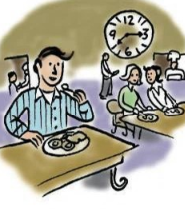
\includegraphics{max_mange.png}
            }
            \only<3-4>{
              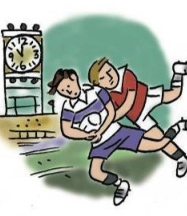
\includegraphics{max_joue.png}
            }
            \only<5-6>{
              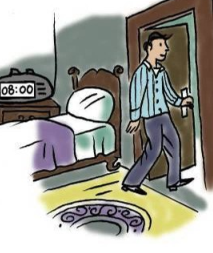
\includegraphics{max_sorti.png}
            }
            \only<7-8>{
              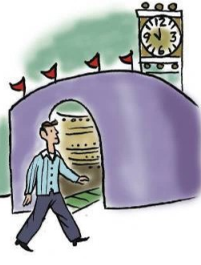
\includegraphics{max_alle.png}
            }
            \only<9-10>{
              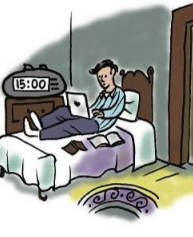
\includegraphics{max_etudie.png}
            }
            \only<11-12>{
              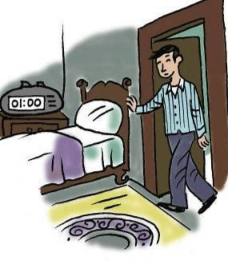
\includegraphics[scale=0.9]{max_rentre.png}
            }
            \only<13->{
              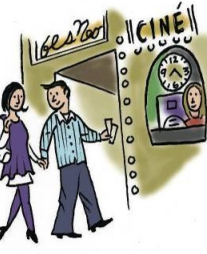
\includegraphics{max_cine.png}
            }
          \end{center}
        \end{minipage}
    \end{columns}
    \uncover<15->{
      \textcolor{green}{D'abord}? \textcolor{red}{Enfin}? \textcolor{orange}{Ensuite, après ou puis}?
    }
  \end{frame}

  \begin{frame}{Ta journée hier}
    Avec un/e partenaire, raconte ce que tu as fait hier.
    Essaie d'utiliser des verbes qui prennent le verbe \lexi{être} au passé composé.
    Ensuite, écris sur le tableau quelles activités vous deux avez faites qui étaient les mêmes en phrases complètes. \\
    \tinygloss{With a partner, describe what you did yesterday.
    Try to use verbs that take the verb \lexi{être} in passé composé.
    Next, write on the board what you both did that was the same using complete sentences.}
    \begin{description}
      \item[] \textbf{Modèle:}
      \item[E1:] Moi, je suis de la maison à 9h.
      \item[E2:] Moi aussi! Après, je suis allée à la fac.
      \item[E1:] Pas moi. Je suis allé chez le dentiste.
      \item[\emph{Tableau:}] Nous sommes sortis de la maison à 9h.
    \end{description}
  \end{frame}

  % \begin{frame}{Mais pourquoi?}
  %    \\
  %   \tinygloss{}
  %   \begin{description}
  %     \item[] \textbf{Modèle:} \emph{}
  %     \item[E1:]
  %   \end{description}
  %   \begin{columns}[t]
  %     \column{0.5\textwidth}
  %       \begin{enumerate}
  %         \item
  %       \end{enumerate}
  %     \column{0.5\textwidth}
  %       \begin{enumerate}
  %         \setcounter{enumi}{}
  %         \item
  %       \end{enumerate}
  %   \end{columns}
  % \end{frame}

  \begin{frame}{}
    \begin{center}
      \Large Questions?
    \end{center}
  \end{frame}
\end{document}
